\chapter{Cristales semiconductores} \label{Ch:09}

Como ya se describió en capítulos anteriores, un semiconductor no es sino un aislantes (a $T=0$K) pero con un gap de energía suficientemente pequeño ($\varepsilon_g <1$ eV) como para que, digamos a temperatura ambiente, una proporción apreciable de la banda de valencia (B.V.) pasan a ocupar la banda de conducción (B.C.). Estos electrones térmicamente excitados y los huecos que dejan de la B.V. pueden transportar corriente eléctrica (figura \ref{Fig:09-01}).


\begin{figure}[h!] \centering
	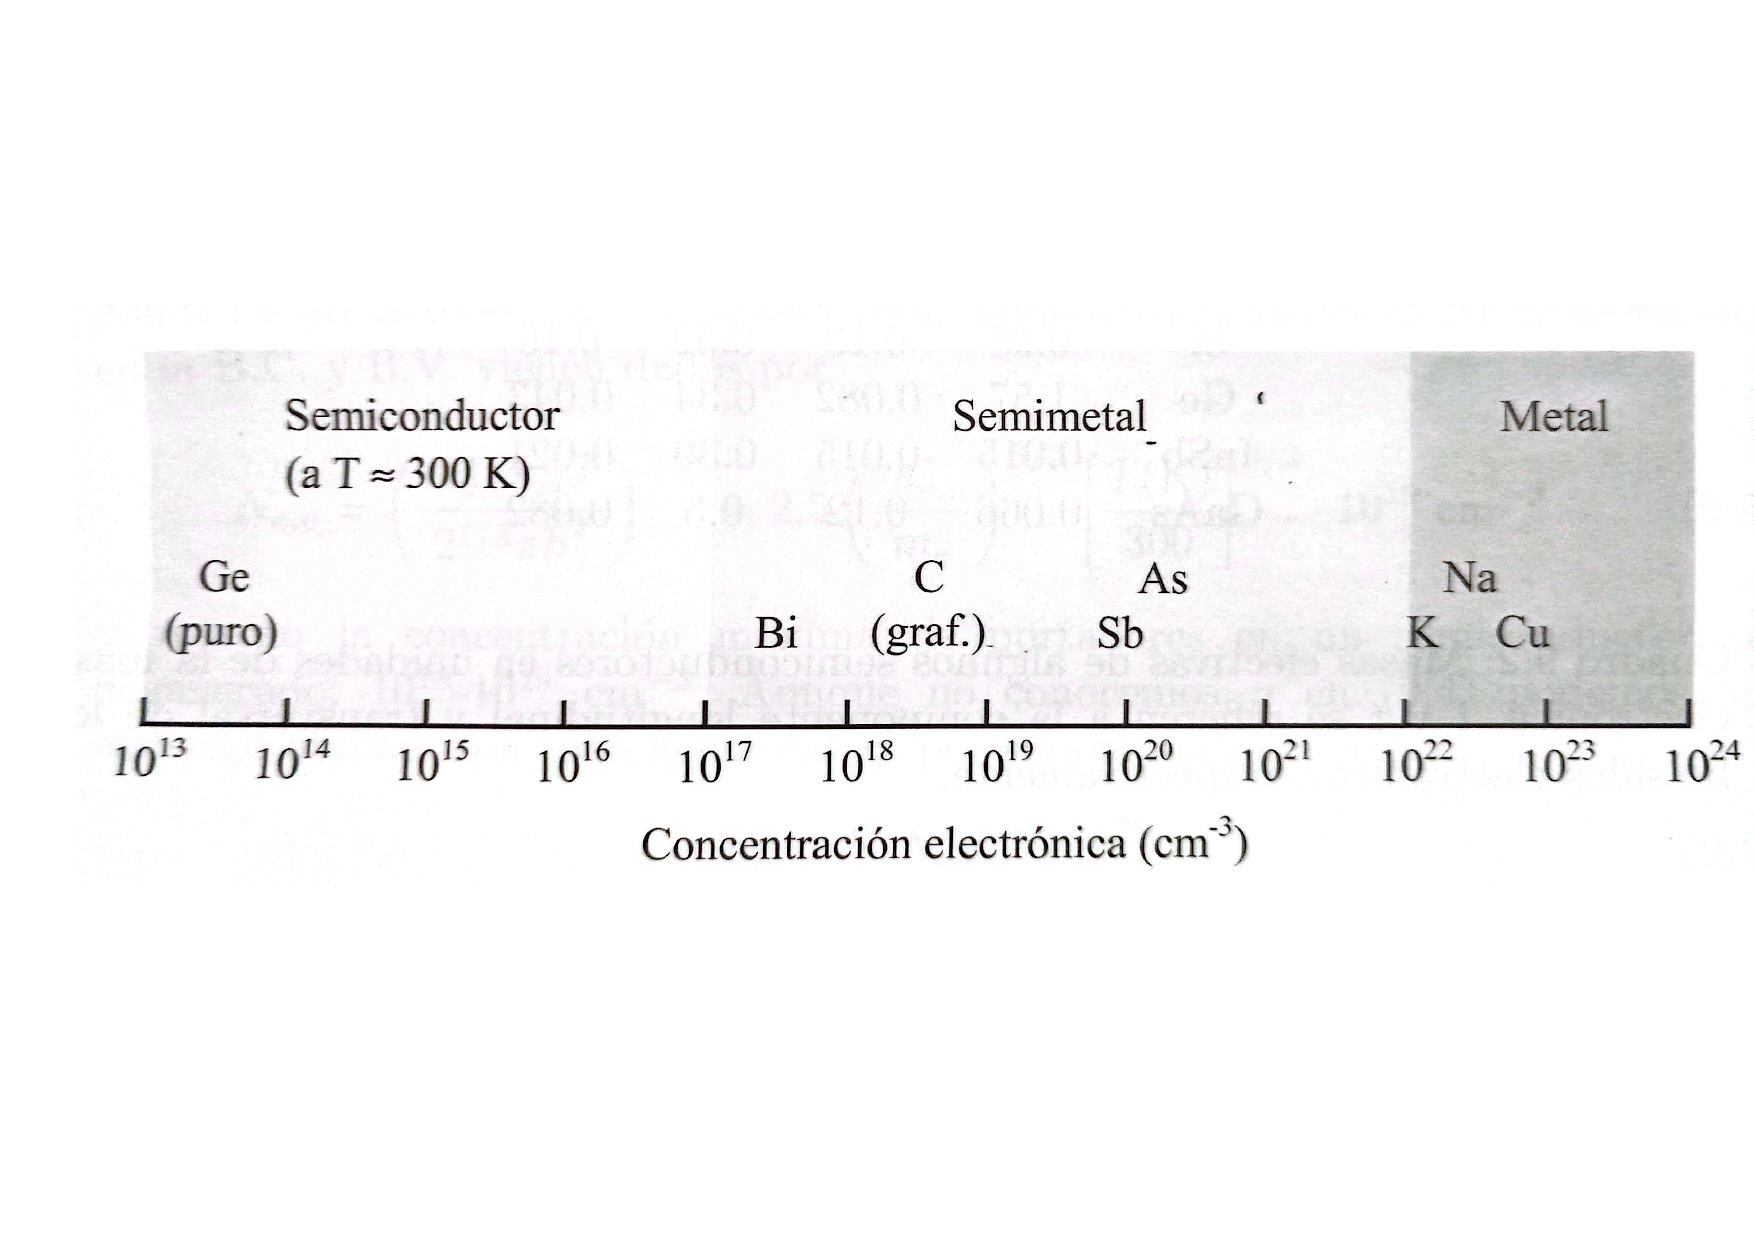
\includegraphics[scale=0.35]{Cuerpo/Ch_09/Fotos libro 1.pdf}
	\caption{Concentración de protadores para algunos metales, semimetales y semiconductores.}
	\label{Fig:09-01}
\end{figure}

Una propiedad especial de los semiconductores, que no se encuentra en metales, es que su conductividad eléctrica se puede alterar en muchos órdenes de manitud añadiendo pequeñas cantidades de otros elementos, que se denominan genéricamente \textit{impurezas}. Éstas determinan el carácter electrón o hueco de la conducción. Toda la electrónica de estado sólido (transistores, conmutadores diodos, células fotovoltaicas, etc.) descansa en esta propiedad conocida como \textit{dopado}.

Los semiconductores son generalmente cristales de enlace covalente. Los más comunes son los del grupo IV y los compuestos de los grupos III-V. El gap de energía $\varepsilon_g$ de algunos materiales se muestra en la tabla \ref{Tab:08-01}. Obsérvese la suave dependencia de $\varepsilon_g$ con la temperatura, debida en parte a la variación del espacio atómico (dilatación).

\begin{table}
\begin{tabular}{ccc}
	Cristal & $\varepsilon_g$ (0 K) & $\varepsilon_g$ (300 K) \\ \hline
	Si & 1.17 & 1.12 \\
	Ge & 0.75 & 0.6 \\
	InSb & 0.23 & 0.17 \\ 
	GaAs & 1.52 & 1.43 \\
	Te & 0.33 & - \\ 
	SiC & 43.0 & - \\
	C (dia) & 5.5 & 5.5
\end{tabular}
\caption{Gap de energía para algunos materiales semiconductores.}
\label{Tab:08-01}
\end{table}
Otro parámetro fundamental es la masa efectiva, algunos de cuyos valores numéricos se muestran en la tabla \ref{Tab:08-02}.

\section{Concetración de portadores en equilibrio térmico}

\section{Semiconductores dopados}

\section{Concentración de portadores en Semiconductores dopados}

\section{Conductividad y movilidad}

\section{Semiconductores inhomogeneos: la unión p-n.}
\begin{figure}[h!] \centering
	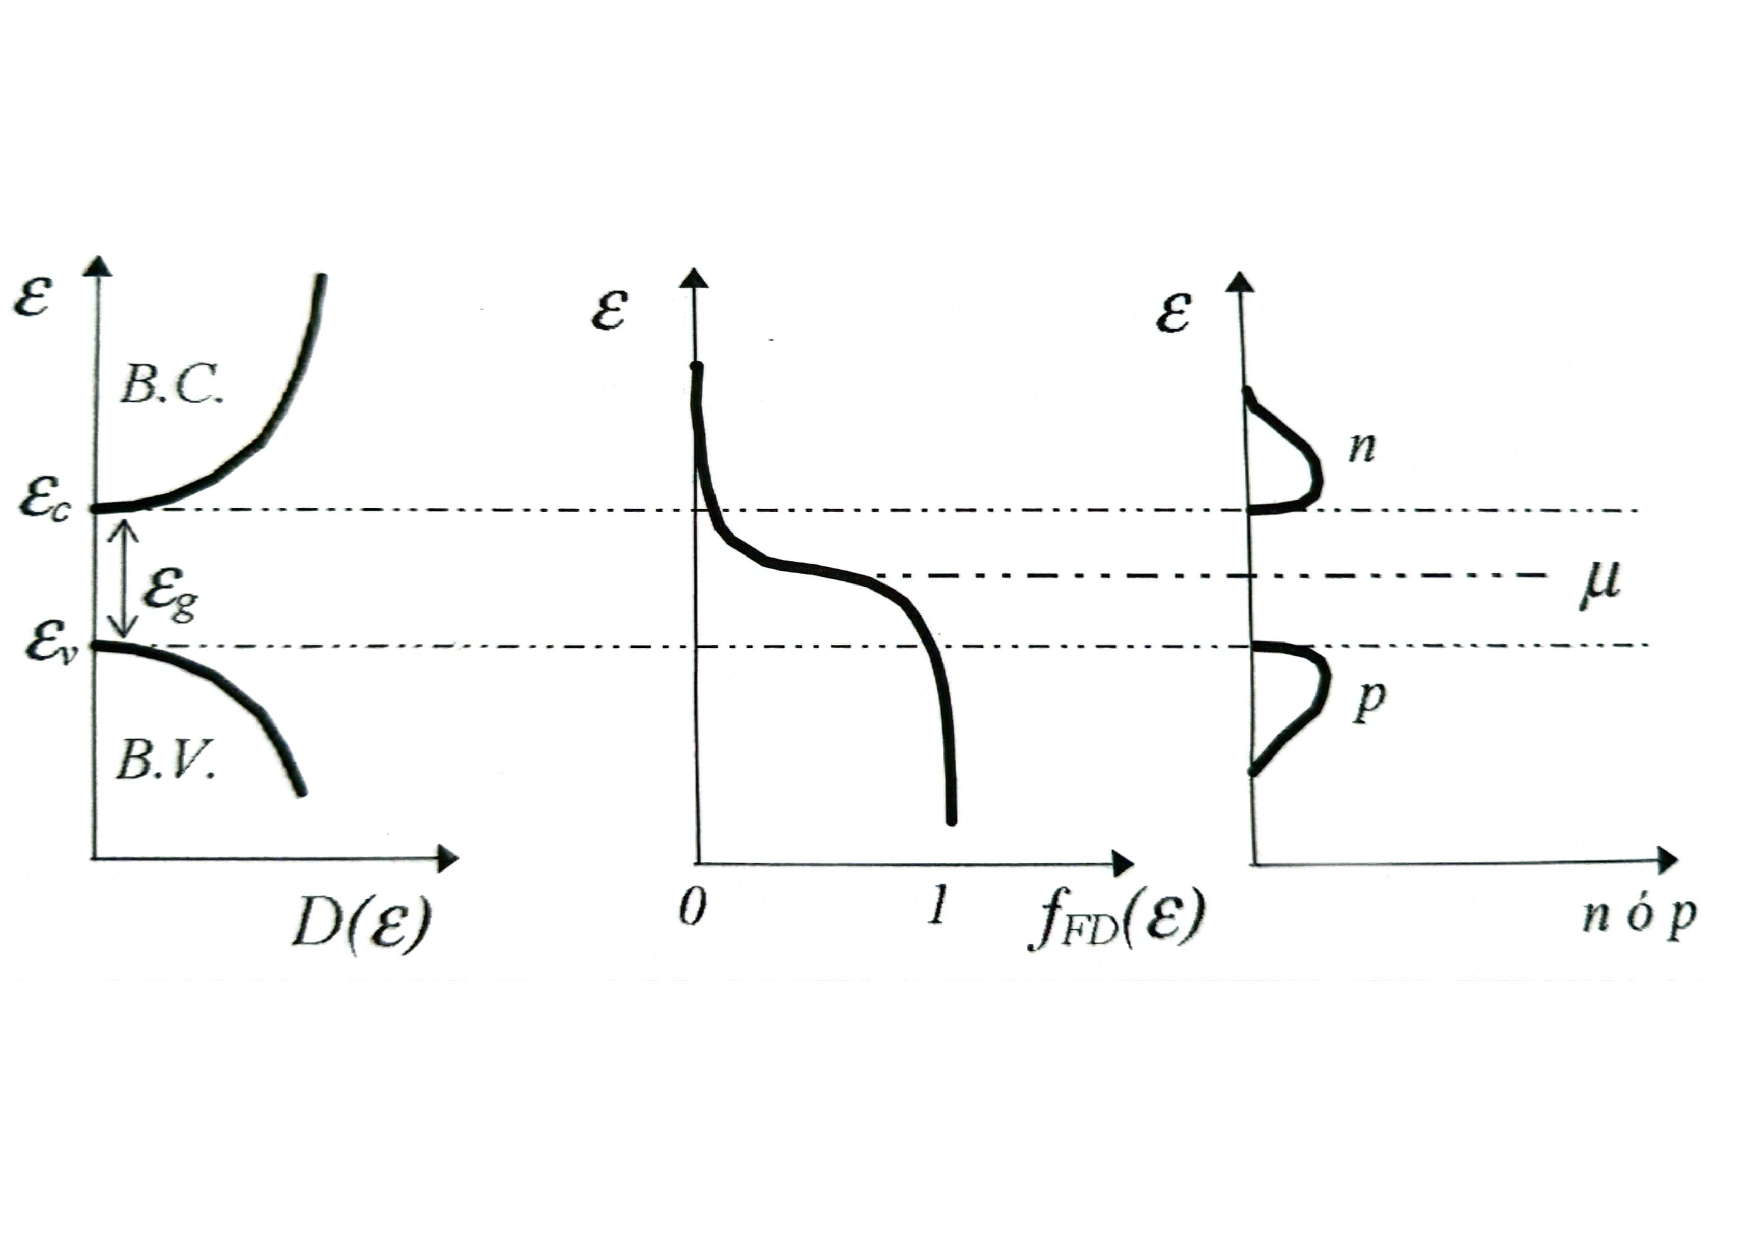
\includegraphics[scale=0.5]{Cuerpo/Ch_09/Fotos libro 2.pdf}
	\caption{}
	\label{Fig:09-02}
\end{figure}
\begin{figure}[h!] \centering
	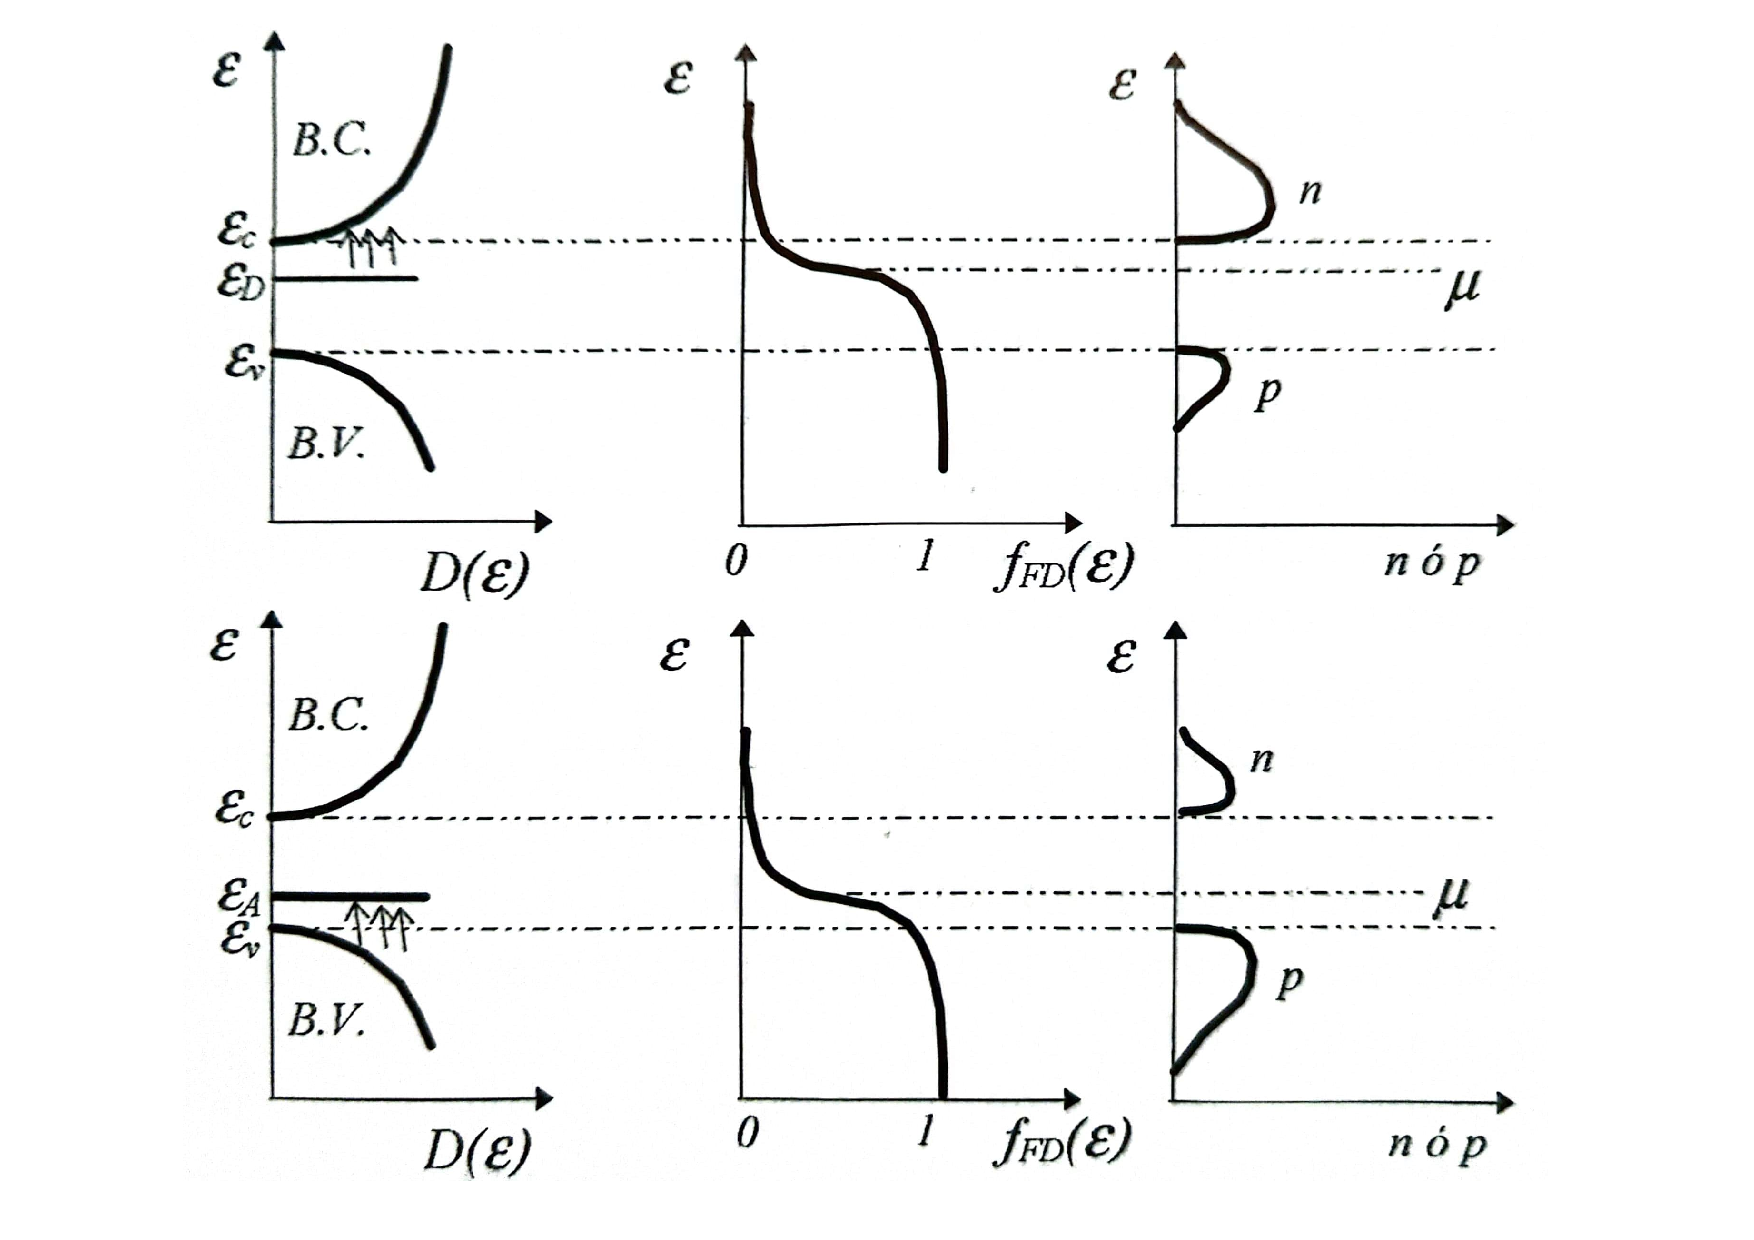
\includegraphics[scale=0.5]{Cuerpo/Ch_09/Fotos libro 3.pdf}
	\caption{}
	\label{Fig:09-03}
\end{figure}
\begin{figure}[h!] \centering
	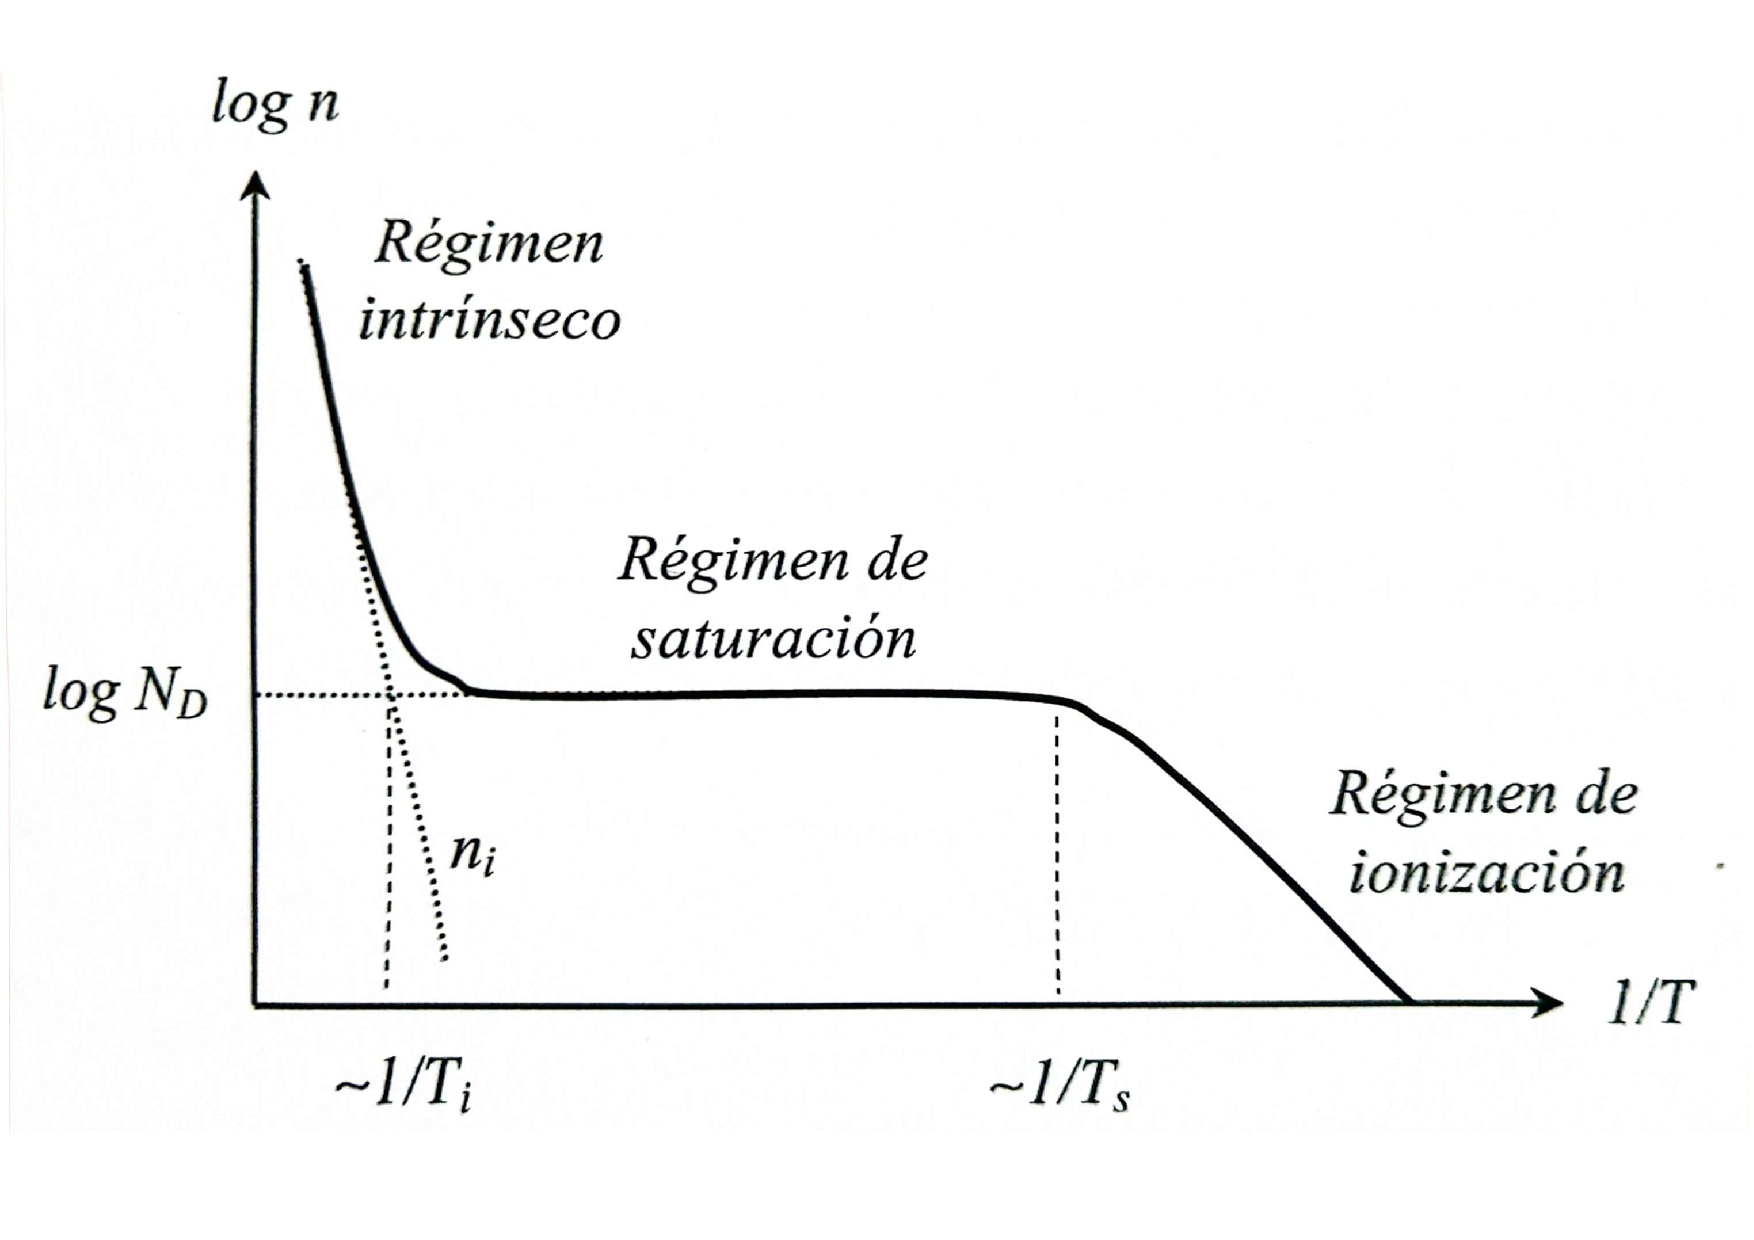
\includegraphics[scale=0.5]{Cuerpo/Ch_09/Fotos libro 4.pdf}
	\caption{}
	\label{Fig:09-04}
\end{figure}
\begin{figure}[h!] \centering
	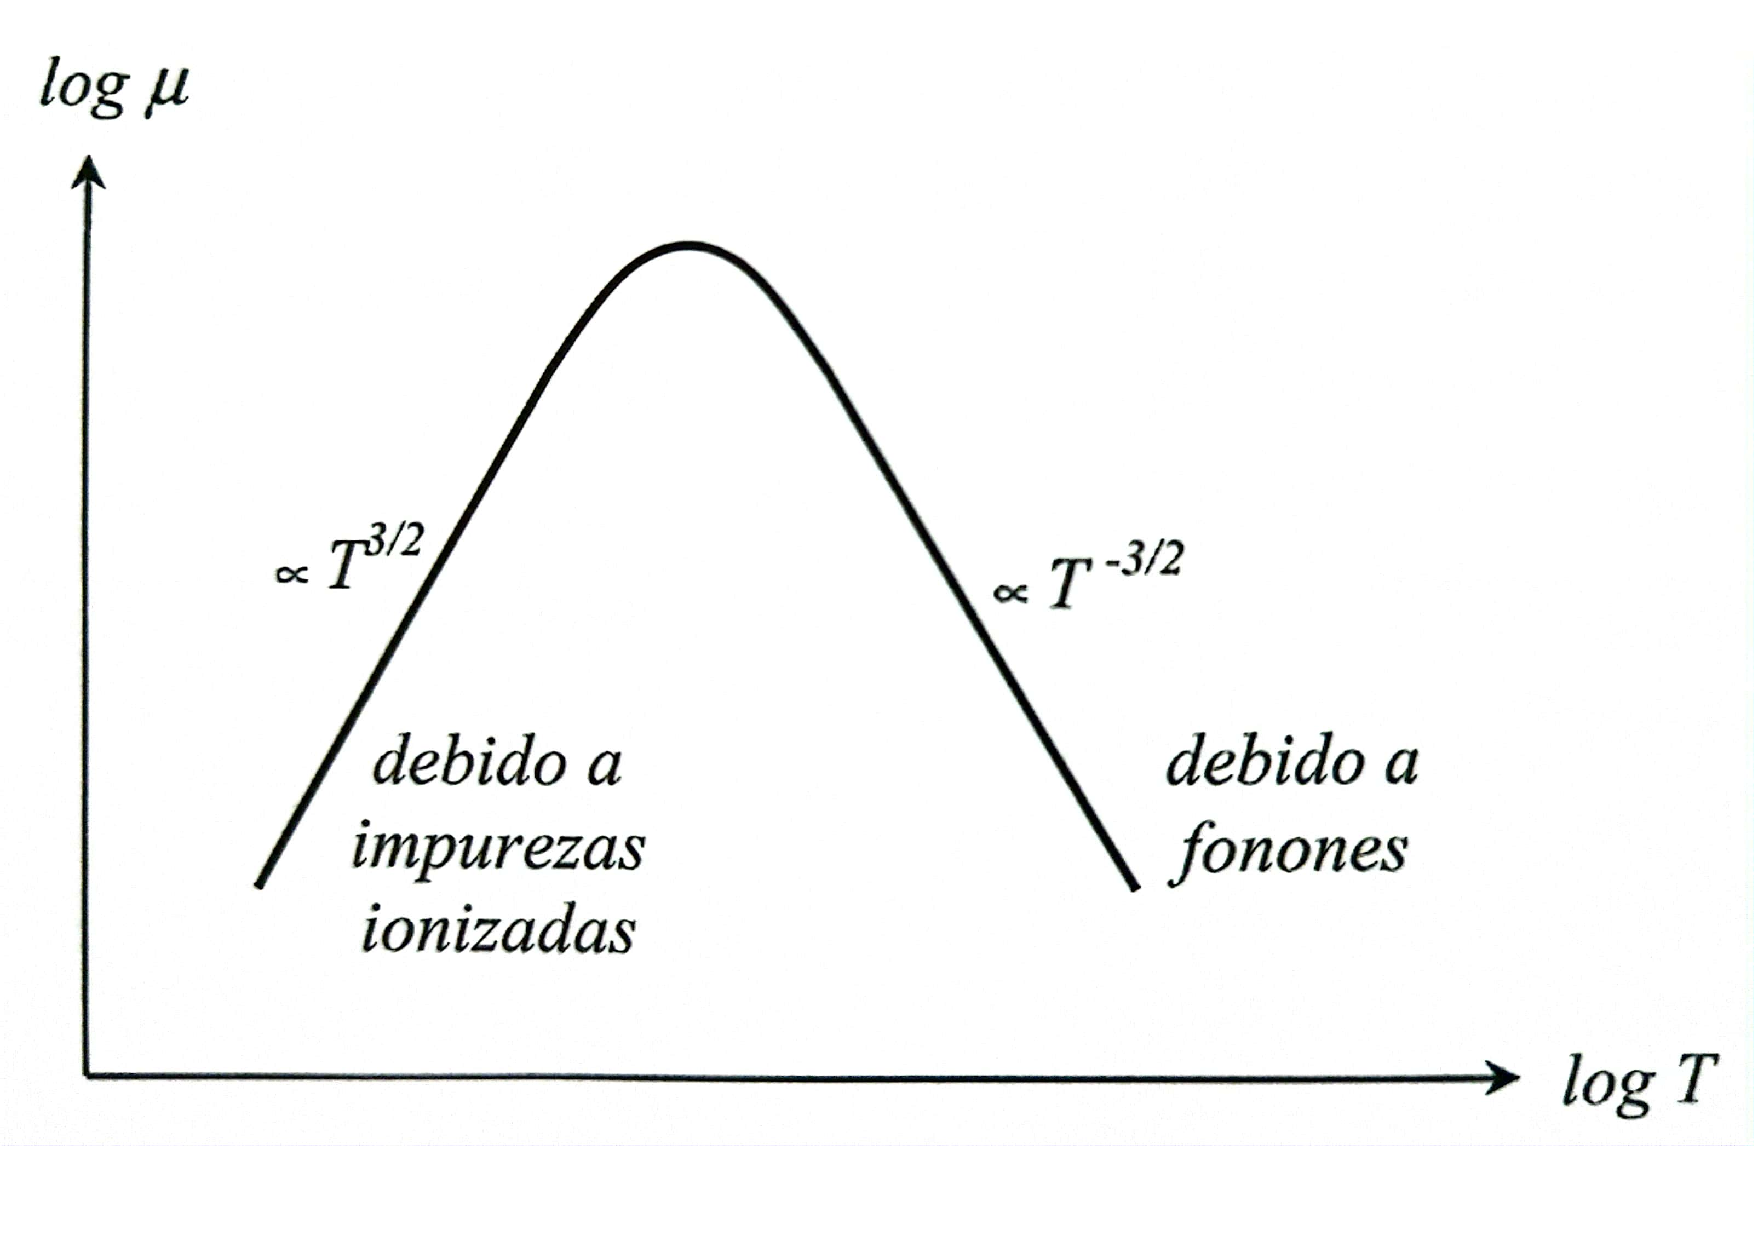
\includegraphics[scale=0.5]{Cuerpo/Ch_09/Fotos libro 5.pdf}
	\caption{}
	\label{Fig:09-05}
\end{figure}
\begin{figure}[h!] \centering
	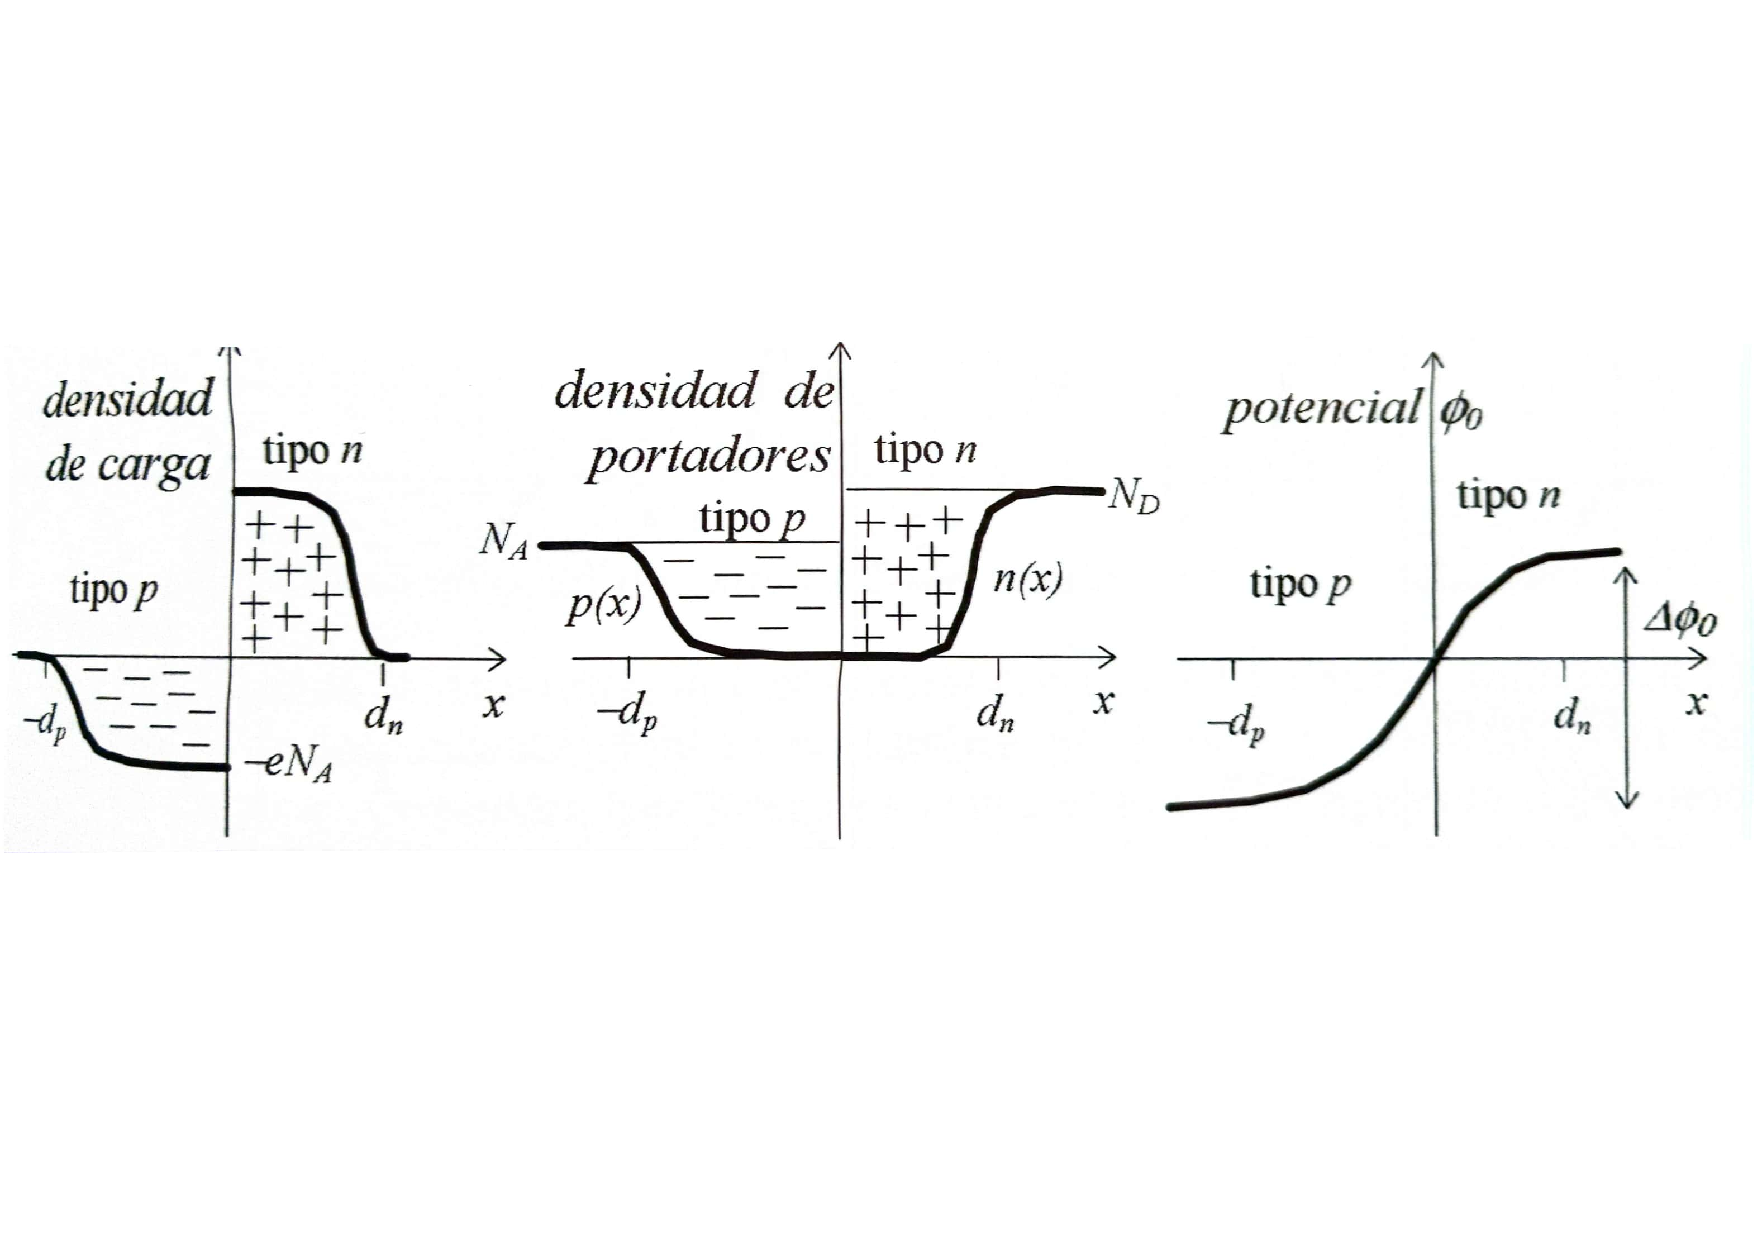
\includegraphics[scale=0.5]{Cuerpo/Ch_09/Fotos libro 6.pdf}
	\caption{}
	\label{Fig:09-06}
\end{figure}
\begin{figure}[h!] \centering
	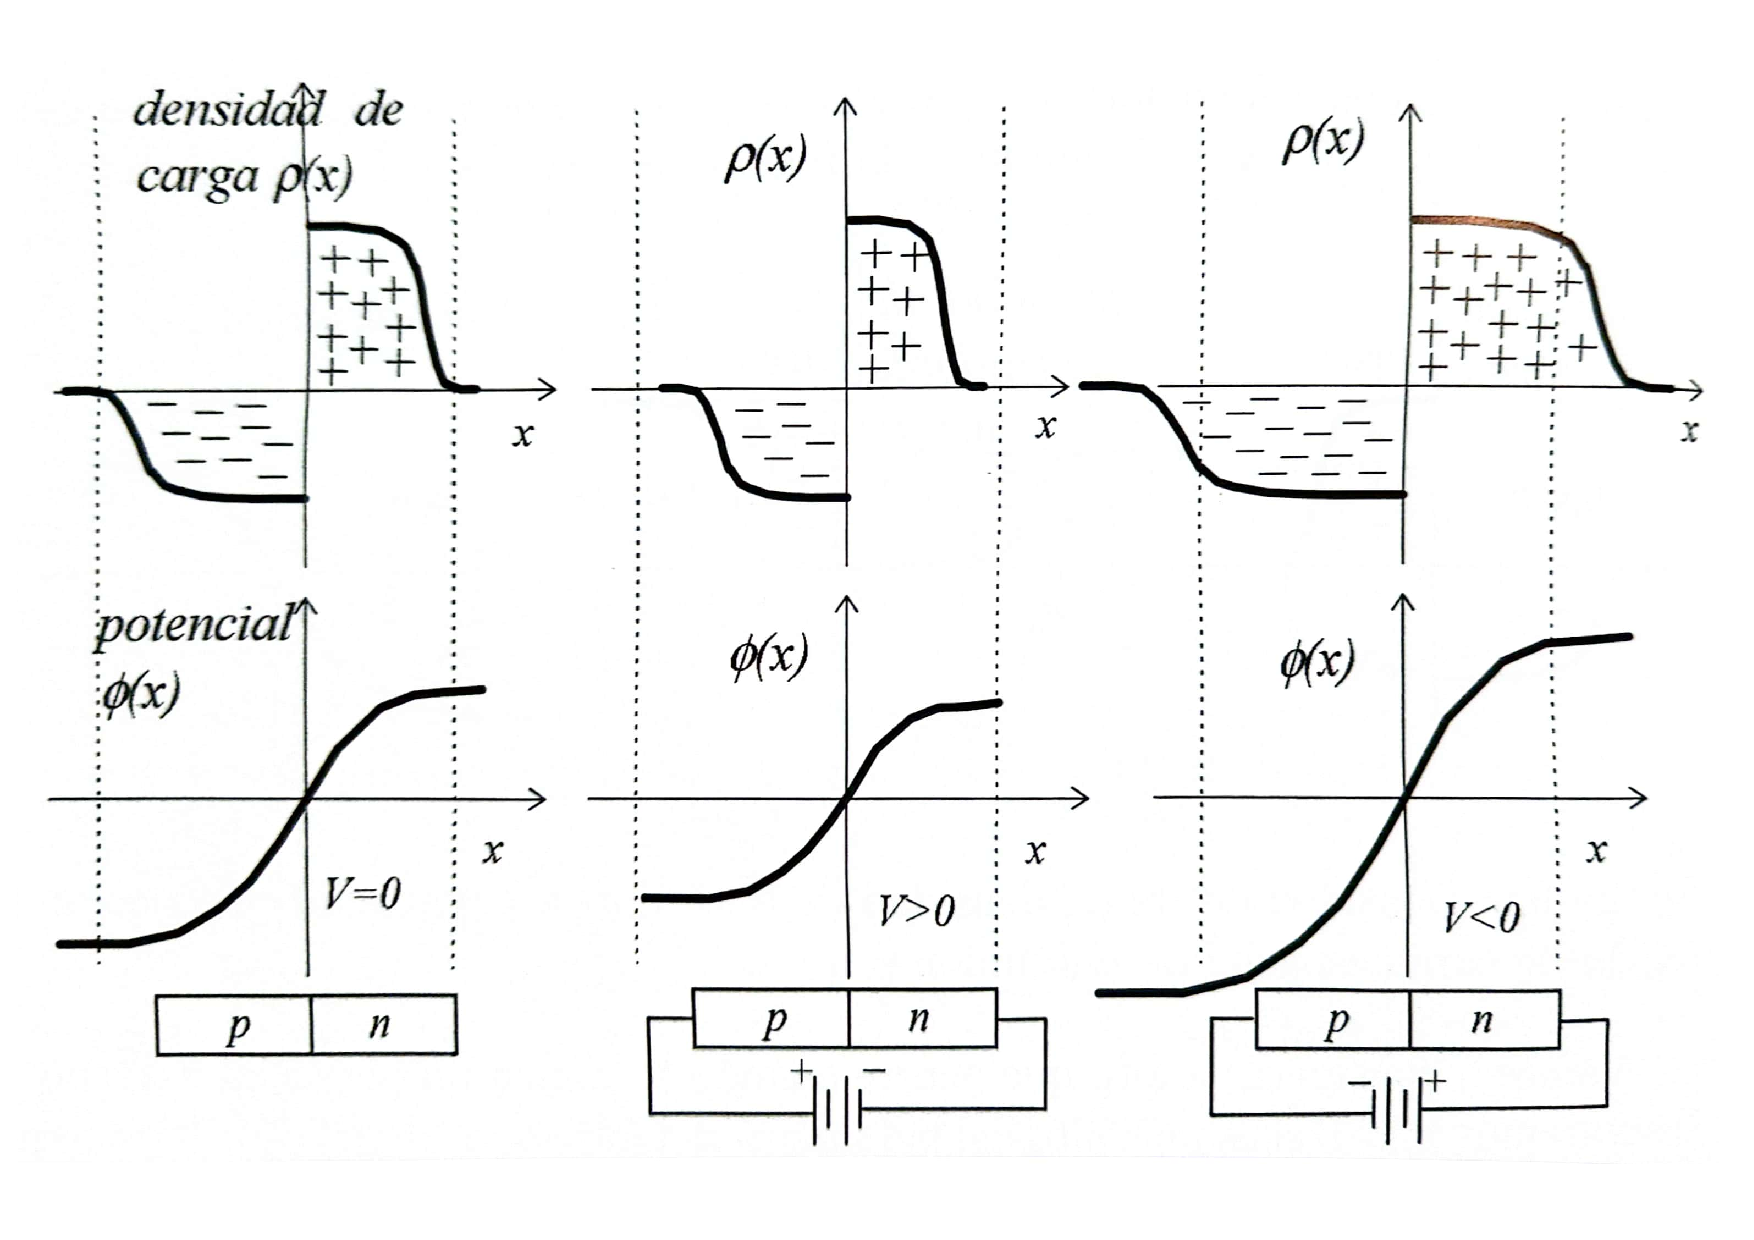
\includegraphics[scale=0.5]{Cuerpo/Ch_09/Fotos libro 7.pdf}
	\caption{}
	\label{Fig:09-07}
\end{figure}
\begin{figure}[h!] \centering
	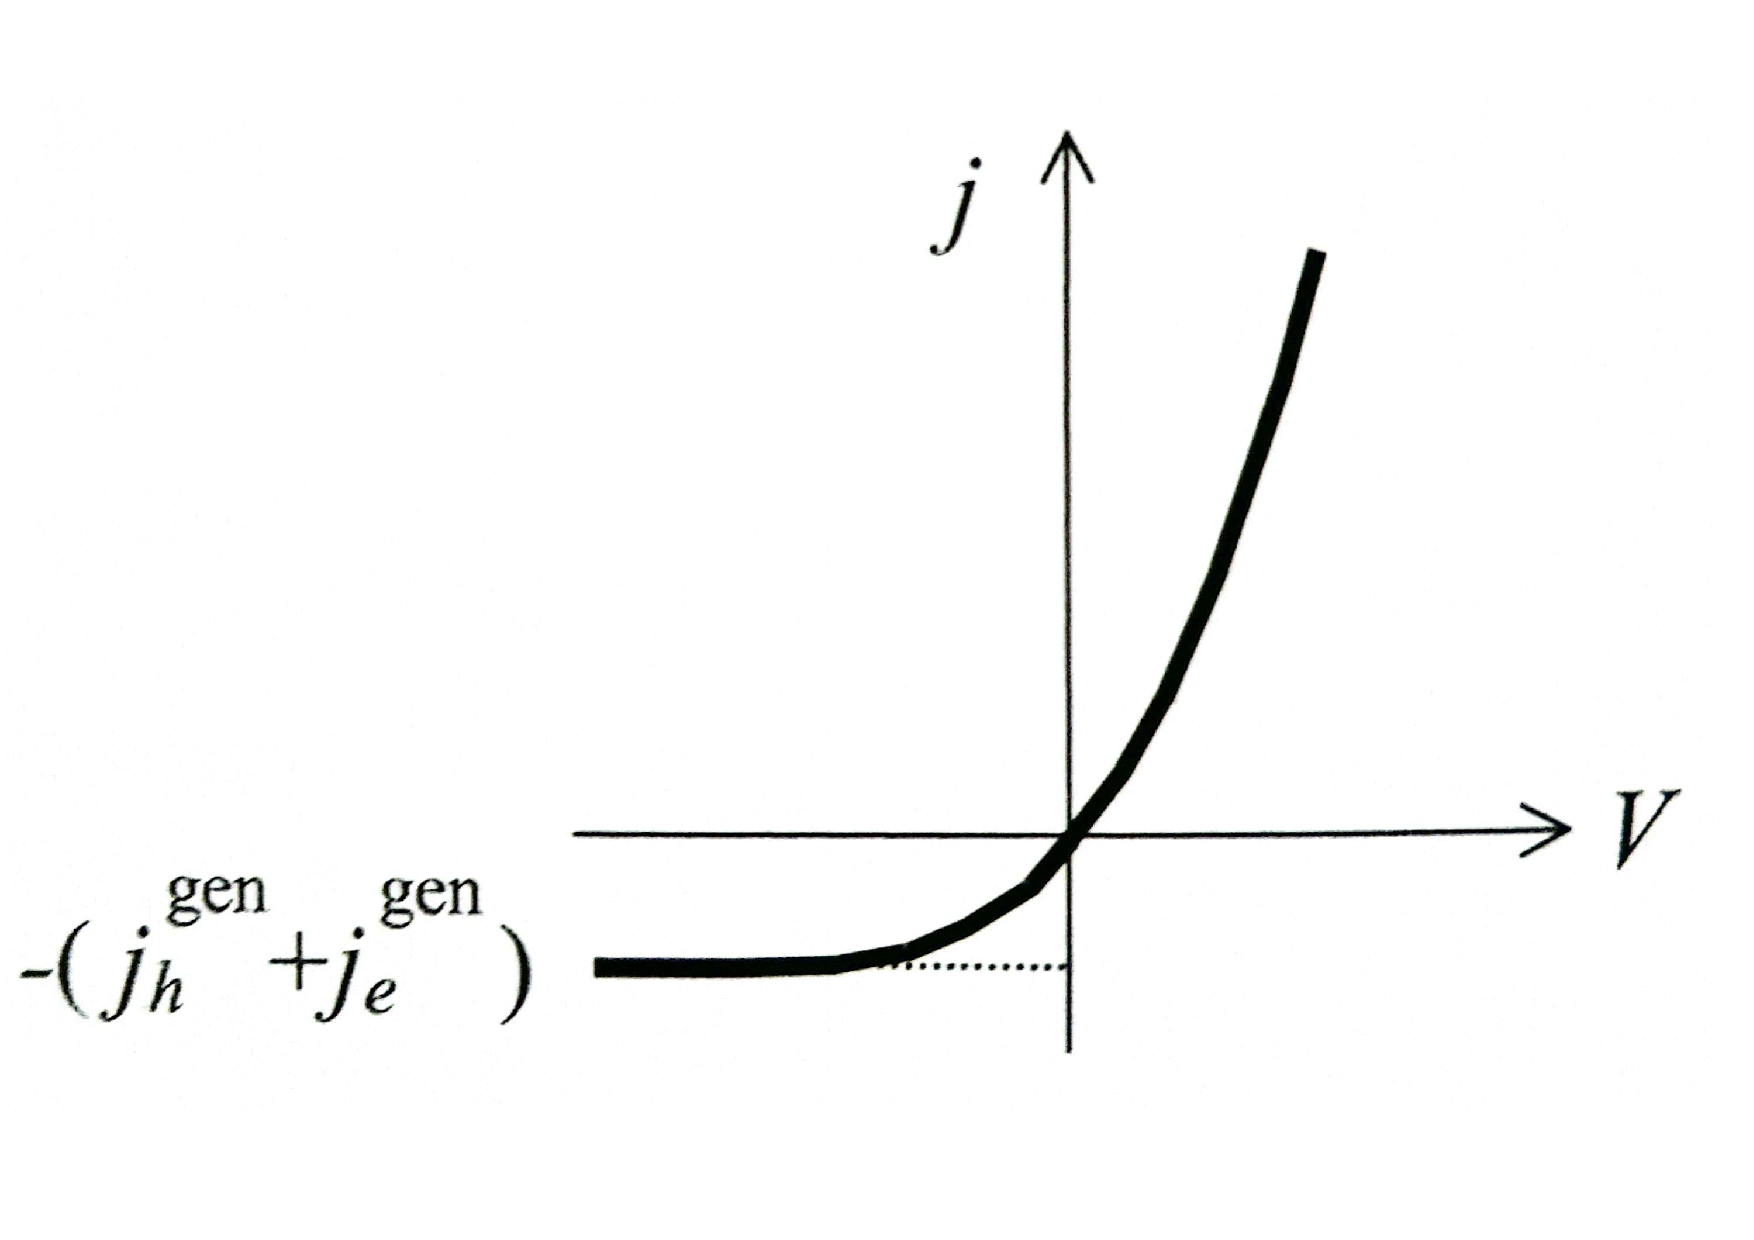
\includegraphics[scale=0.5]{Cuerpo/Ch_09/Fotos libro 8.pdf}
	\caption{}
	\label{Fig:09-08}
\end{figure}